Several generic queries have also been executed on both the Data Warehouse and the on-premise databases.
These queries present different properties, and are representative of the actual workload.

The execution times of these queries have been recorded and compared.

\subsubsection{Query types}
    Specific queries have been developed to test different usage scenarios.
    
    These queries are:
    \paragraph{Count}
        This query needs to count how many rows are in a table.
        It requires a scan of the whole table, but access to no values.
    
    \paragraph{Generic selection}
        This query is expected to perform a sequential scan of the table and return all values.
        The speed of this query depends solely on the database power.
        
    \paragraph{Low selectivity}
        This query has a simple \code{WHERE} clause, which is expected to retrieve around 50\% of the data.
        
    \paragraph{High selectivity}
        This query has a more complex \code{WHERE} clause ranging over multiple attributes.
        It is expected to retrieve a small amount of data.
        
    \paragraph{Ordering}
        This query retrieves a medium-sized dataset and is tasked with sorting it according to a given value.
        
    \paragraph{Aggregation}
        This test divides the data into groups and computes an aggregated value for each group.
        
    \paragraph{Duplicate removal}
        This query selects a large number of rows and tries to remove all duplicate from multiple columns.
        
    \paragraph{Insertion / Deletion}
        Two similar queries insert a medium amount of rows in a table and then remove them.
        Times are recorded independently for insertion and deletion.
        
\subsubsection{Table types}
    \textit{Azure SQL Data Warehouse} supports three different table types, offering different indexing options \cite{bib:tests:perf:indexing}.
    
    Tests have been carried out on all three types, to serve both as a comparison between different options and to give a more precise estimation of the improvements provided by the Data Warehouse.
    
    \paragraph{Heap tables}
        Heap tables are optimized for insertion and deletion operations.
        
        Rows are stored in the order in which they are inserted into the table, although the Database Engine can move data around in the heap to increase the storage efficiency \cite{bib:tests:perf:heap}.
        
        As a consequence, the data order cannot be predicted. Clustering indexes cannot be applied to heap tables.
        
    \paragraph{Column-store index tables}
        Column-store tables store data as columns, as opposed to the traditional row storage \cite{bib:tests:perf:columnstore}.
        
        This storage type allows very fast access to multiple rows of a single column, since they are stored in the same memory block.
        Additionally, only the selected columns are fetched, avoiding retrieval of unnecessary data.
        
        Column-store tables can be either clustered or non-clustered.
        The former allows specifying only a single clustering column.
        
    \paragraph{Clustered index tables}
        Clustered tables store data in sorted order, depending on the clustering index chosen.
        They are very efficient for retrieving sorted data and for performing selection operations on the cluster index.
        
        On the other hand, sorting operation of different attributes may be penalized, compared to other table type.
        Insertion and deletion operation need to update the clustering index each time, creating additional overhead.
        
\subsubsection{Setup}
    The queries have been executed on both databases on identical tables, having the both same structure and data.
    
    \paragraph{Measurements}
        \begin{figure}
            \centering
            \fbox{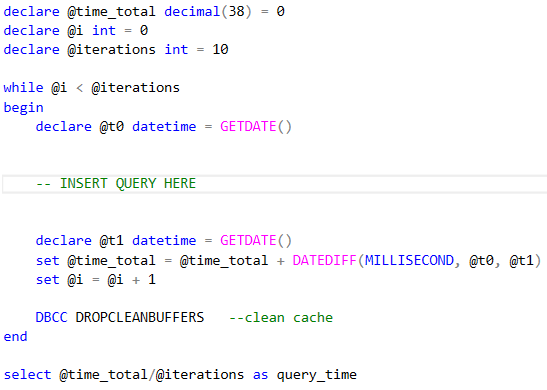
\includegraphics[width=.7\textwidth]{res/tests/sql_wrapper.png}}
            \caption{SQL wrapper for collecting accurate query execution time.}
            \label{fig:tests:perf:queries:wrapper}
        \end{figure}
    
        A small SQL wrapper for the query, shown in Figure \ref{fig:tests:perf:queries:wrapper}, has been created in order to collect accurate measurements.
        
        This wrapper records both the starting and ending time of the query, from which the actual execution time can be computed.
        
        Multiple executions of the same queries are performed in order to improve result accuracy.
        The resulting execution time is the average of all the times obtained.
        
    \paragraph{Caching}
        Databases can cache query results to speed up successive executions of the same query.
        
        Although caching improves query performance, it can produce misleading results in our tests, since we are going to execute the same query many times in a row.
        
        It is impossible to disable result caching for a specific query, but it is possible to clean up the whole cache, preventing it from invalidating test results.
        